\documentclass{article}

\usepackage{graphicx}
\usepackage{tikz}
\usepackage{tikzsymbols}
\usetikzlibrary{calc,patterns,shapes.geometric}
\pagestyle{empty}
\usepackage[margin=0pt]{geometry}
\geometry{papersize={14in,12in}}

\def\centerarc[#1](#2)(#3:#4:#5){\draw[#1] ($(#2)+({#5*cos(#3)},{#5*sin(#3)})$) arc (#3:#4:#5);}

\begin{document}
	\begin{figure}
		\centering
		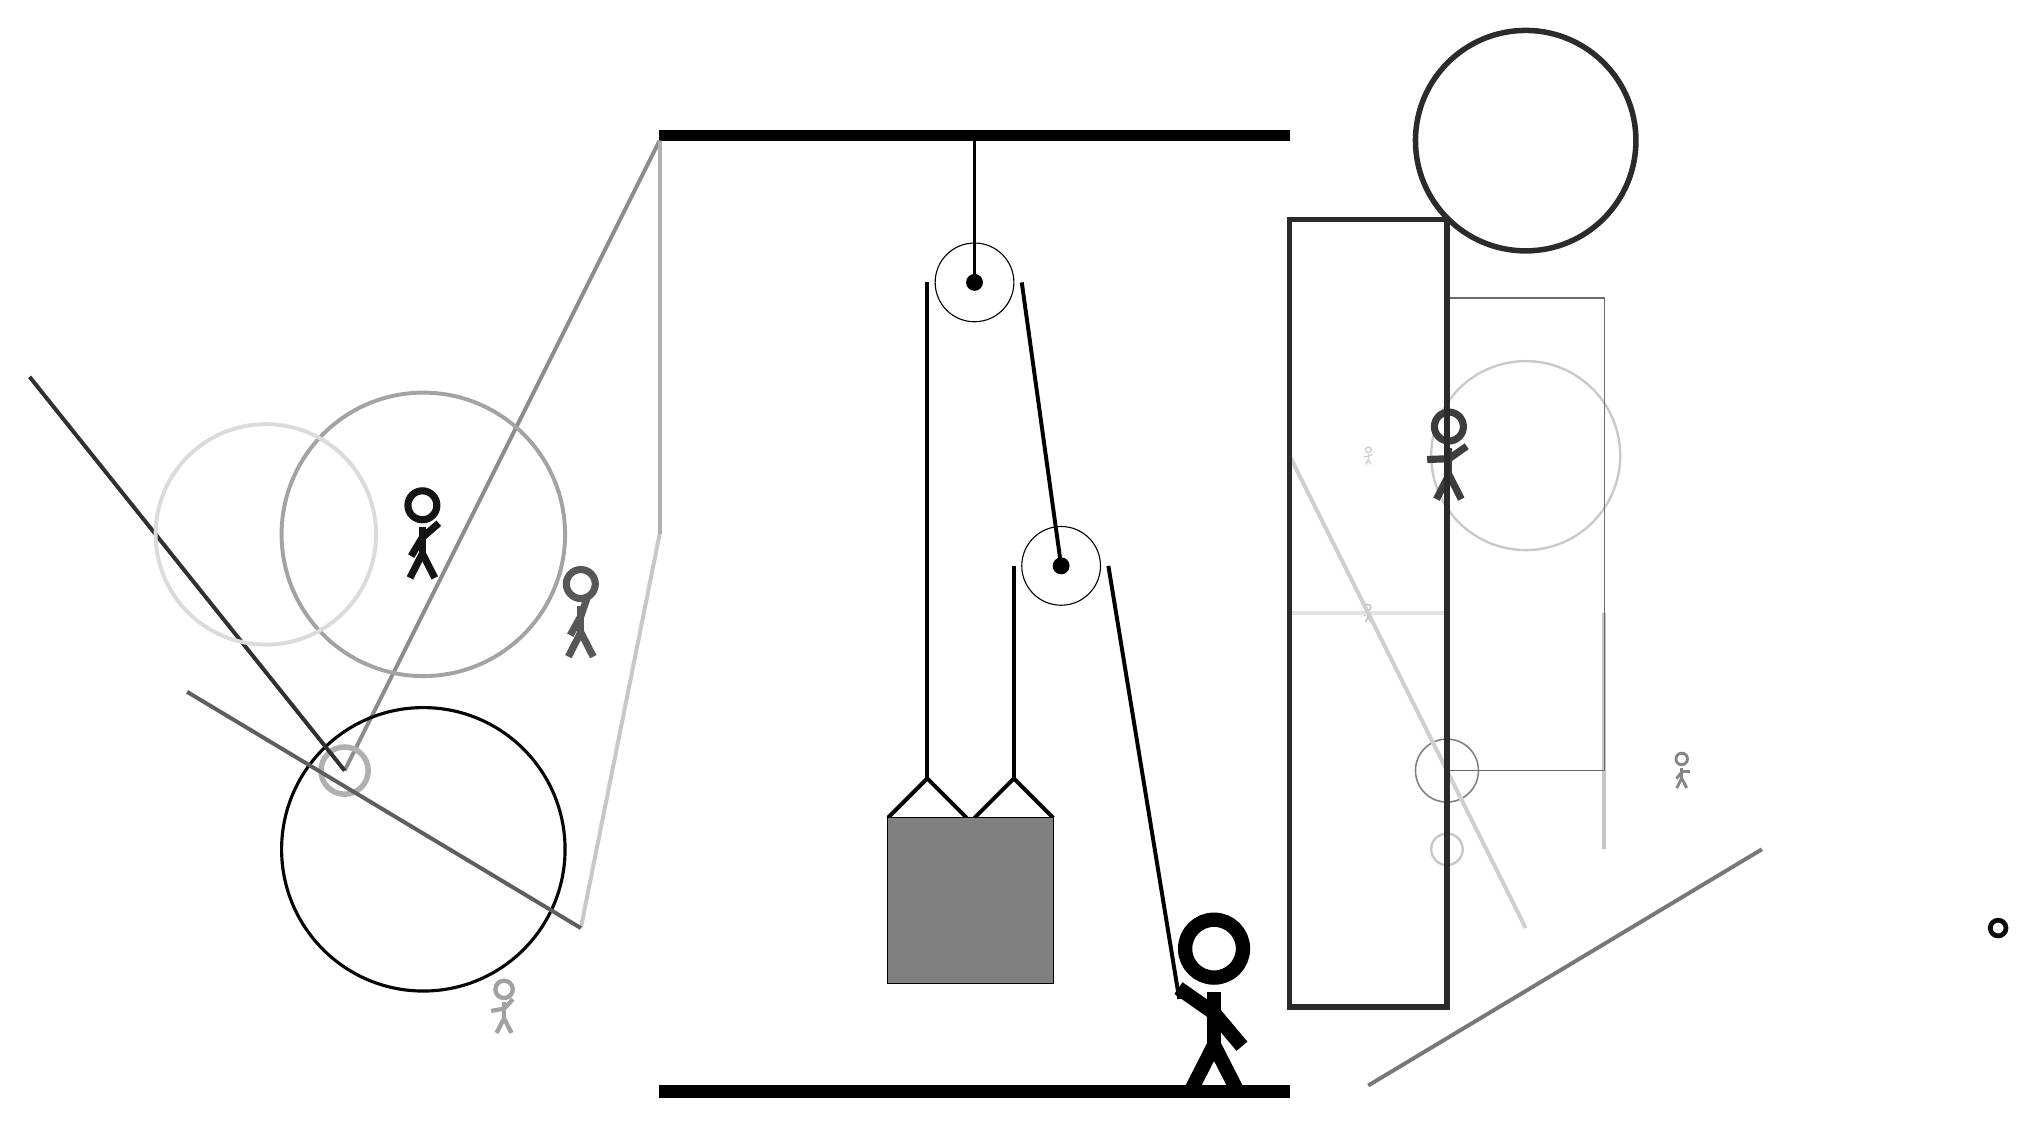
\begin{tikzpicture}
			%%%%% START %%%%%
			
			\draw[fill=black] (-2, 9) rectangle (6, 9.125);
			
			\draw (2, 7.2) circle (0.5);
			\draw[fill=black] (2, 7.2) circle (0.1);
			\draw[thick] (2, 7.2) -- (2, 9);
			
			\draw[line width=0.5mm, color=black!83] (8, 0) rectangle (8, 5);
			
			\draw[line width=0.5mm, color=black!45](-6, 1) -- (-2, 9);
			\node[line width=0.5mm, color=black!19] at (7, 5) {\Strichmaxerl[1][8][23]};
			\draw[line width=0.5mm, color=black!22](-2, 4) -- (-3, -1);
			
			\draw [line width=0.3mm, color=black!37](-7, 4) circle (1.4);
			\draw [line width=0.3mm, color=black!21](9, 5) circle (1.2);
			\node[line width=0.4mm, color=black!26] at (7, 3) {\Strichmaxerl[1][24][7]};
			
			\draw [line width=0.4mm, color=black!98](-5, 0) circle (1.8);
			\node[line width=0.6mm, color=black!37] at (-4, -2) {\Strichmaxerl[3][10][47]};
			\draw [line width=0.5mm, color=black!41](11, 3) circle (0.0);
			
			\draw[line width=0.5mm, color=black!11] (8, 3) rectangle (6, 3);
			
			\draw [line width=0.2mm, color=black!50](8, 1) circle (0.4);
			\draw[line width=0.5mm, color=black!53](7, -3) -- (12, 0);
			
			\draw [line width=0.7mm, color=black!31](-6, 1) circle (0.3);
			\draw[line width=0.5mm, color=black!23](10, 3) -- (10, 0);
			\draw [line width=0.3mm, color=black!22](8, 0) circle (0.2);
			
			\node[line width=0.6mm, color=black!48] at (11, 1) {\Strichmaxerl[2][53][0]};
			\draw [line width=0.7mm, color=black!83](9, 9) circle (1.4);
			\node[line width=0.7mm, color=black!92] at (-5, 4) {\Strichmaxerl[5][59][41]};
			\node[line width=0.6mm, color=black!76] at (8, 5) {\Strichmaxerl[5][2][35]};
			\draw[line width=0.5mm, color=black!81](-6, 1) -- (-10, 6);
			
			\draw[line width=0.5mm, color=black!19](9, -1) -- (6, 5);
			
			\draw[line width=0.2mm, color=black!58] (8, 1) rectangle (10, 7);
			\draw [line width=0.6mm, color=black!96](15, -1) circle (0.1);
			\draw[line width=0.7mm, color=black!83] (6, -2) rectangle (8, 8);
			\draw [line width=0.5mm, color=black!36](-5, 4) circle (1.8);
			\draw [line width=0.5mm, color=black!14](-7, 4) circle (1.4);
			\node[line width=0.3mm, color=black!66] at (-3, 3) {\Strichmaxerl[5][61][71]};
			\draw[line width=0.5mm, color=black!31] (-2, 9) rectangle (-2, 4);
			\draw[line width=0.5mm, color=black!63](-3, -1) -- (-8, 2);
			
			\draw (3.1, 3.6) circle (0.5);
			\draw[fill=black] (3.1, 3.6) circle (0.1);
			
			\draw[line width = 0.5mm]  (0.9, 0.4) -- (1.4, 0.9) -- (1.9, 0.4);
			\draw[line width = 0.5mm]  (2.0, 0.4) -- (2.5, 0.9) -- (3.0, 0.4);
			\draw[fill=black!50] (0.9, 0.4) rectangle (3.0, -1.7);
			
			\draw[line width = 0.5mm] (1.4, 7.2) -- (1.4, 0.9);
			\centerarc[line width = 0.5mm](2, 7.2)(0:180:0.6);
			\draw[line width = 0.5mm] (2.6, 7.2) -- (3.1, 3.6);
			\draw[line width = 0.5mm] (2.5, 3.6) -- (2.5, 0.9);
			\centerarc[line width = 0.5mm](3.1, 3.6)(0:180:0.6);
			\draw[line width = 0.5mm] (3.7, 3.6) -- (4.6, -1.9);
			
			\node at (5, -2) {\Strichmaxerl[10][-35][-50]};
			
			\draw[fill=black] (-2, -3) rectangle (6, -3.15);
			
			%%%%% END %%%%%
		\end{tikzpicture}
	\end{figure}	
\end{document}